\documentclass[a4paper,12pt]{report}
% book report(no part) article(no part/section) letter slides
%      ------          -------
% chapter c section c subsection c subsubsection c paragraph c subparagraph

% ----------------------------------
% PACKAGES
% ----------------------------------

% \usepackage[noTeX]{mmap}
\usepackage{cmap}
\usepackage[T1,T2A]{fontenc}
\usepackage[utf8]{inputenc}
% \usepackage{hyphsubst}
\usepackage[english,russian]{babel}
\usepackage[left=1in,right=1in,top=1in,bottom=1in,paper=a4paper]{geometry}
\usepackage{amsmath,amsfonts,amsthm,amssymb,mathtools}
\usepackage{lipsum}
% \usepackage{extsizes} -- conflict with geometry package
\usepackage{xfrac}
\usepackage{enumitem}
\usepackage{bookmark}

% ----------------------------------
% custom packages
% \usepackage{bigints}
% ----------------------------------

\usepackage{hyperref,theoremref}
\usepackage{cleveref}
\usepackage{nameref}
\hypersetup{
    colorlinks=true,
    linkcolor=blue,
    filecolor=magenta,
    urlcolor=blue,
    pdftitle={assignment},
}
\urlstyle{same}
\newcommand\myref[1]{\hyperref[#1]{#1}}

\usepackage{etoolbox}
\usepackage{multicol,array}
\usepackage{pdfpages}

\usepackage{graphicx}
\graphicspath{ {./graphics/} }

\mathtoolsset{showonlyrefs=false}
% \usepackage{leqno}

\usepackage{biblatex}
% \usepackage{cite}
\usepackage{csquotes}
% \renewcommand{\refname}{Список источников}  % default: "Список литературы" (article)
% \renewcommand{\bibname}{Список литературы} % default: "Литература" (book и report)


% ----------------------------------
% COMMANDS
% ----------------------------------

% bigcdot ( \cdot < \bigcdot < \bullet )
\makeatletter
\newcommand*\bigcdot{\mathpalette\bigcdot@{.5}}
\newcommand*\bigcdot@[2]{\mathbin{\vcenter{\hbox{\scalebox{#2}{$\m@th#1\bullet$}}}}}
\makeatother

% deliminator
\DeclarePairedDelimiter{\abs}{\lvert}{\rvert}
\DeclarePairedDelimiter{\norm}{\lVert}{\rVert}
\DeclarePairedDelimiter{\ceil}{\lceil}{\rceil}
\DeclarePairedDelimiter{\floor}{\lfloor}{\rfloor}
\DeclarePairedDelimiter{\round}{\lfloor}{\rceil}

\usepackage[dvipsnames, table, xcdraw]{xcolor} % load before pgfplots
\usepackage{pgfplots}
\pgfplotsset{compat=1.18}
\usepackage{tikz}
\usetikzlibrary{positioning}
\usetikzlibrary{arrows.meta}
\usetikzlibrary{decorations.pathreplacing,calligraphy}
\usetikzlibrary{shapes.geometric}
\usepgfplotslibrary{colorbrewer}
\usepackage[export]{adjustbox}
\usepackage{subfig}

\usepackage{listings}
\usepackage{fontawesome}
\usepackage{minted}

% \usepackage{tcolorbox}
% \BeforeBeginEnvironment{code}{\begin{tcolorbox}}%
% \AfterEndEnvironment{code}{\end{tcolorbox}}%
    % \renewcommand\listingscaption{My Listing Caption}

\setminted{
    frame=lines,
    linenos=true,
    autogobble,
}

% \renewcommand{\lstlistlistingname}{Список листингов}
% put it ^^^ just before \lstlistoflistings
\renewcommand{\lstlistingname}{Листинг}
\newenvironment{code}{\captionsetup{type=lstlisting}}{}
% \renewcommand{\lstlistlistingname}{Список листингов}


% \lstset{
%      backgroundcolor=\color{gray!10},
% }
%
% \DeclareCaptionFont{white}{\color{white}}
% \DeclareCaptionFormat{listing}{\colorbox{gray!90}{\parbox{\dimexpr\linewidth-2\fboxsep\relax}{#1#2#3}}}
% \captionsetup[lstlisting]{format=listing,labelfont=white,textfont=white,justification=centering}



% \begin{lstlisting}[label=some-code,caption=Some Code]
%     public void here() {
%         goes().the().code()
%     }
% \end{lstlisting}

% https://tex.stackexchange.com/questions/107516/minted-customise-listing-name
% https://stackoverflow.com/questions/741985/latex-source-code-listing-like-in-professional-books

\usepackage{biblatex}
% \usepackage{cite}
\usepackage{csquotes}
% \renewcommand{\refname}{Список источников}  % default: "Список литературы" (article)
% \renewcommand{\bibname}{Список литературы} % default: "Литература" (book и report)

% ----------------------------------
% range [a,b]
% ----------------------------------
\newcommand\abseg{\ensuremath{[a,b]}}
\newcommand\abint{\ensuremath{(a,b)}}

% ----------------------------------
% bigcdot ( \cdot < \bigcdot < \bullet )
% ----------------------------------
\makeatletter
\newcommand*\bigcdot{\mathpalette\bigcdot@{.5}}
\newcommand*\bigcdot@[2]{\mathbin{\vcenter{\hbox{\scalebox{#2}{$\m@th#1\bullet$}}}}}
\makeatother

% ----------------------------------
% argmax, argmin
% ----------------------------------
\DeclareMathOperator*{\argmax}{argmax}
\DeclareMathOperator*{\argmin}{argmin}

% ----------------------------------
% deliminator
% ----------------------------------
\DeclarePairedDelimiter{\abs}{\lvert}{\rvert}
\DeclarePairedDelimiter{\norm}{\lVert}{\rVert}
\DeclarePairedDelimiter{\ceil}{\lceil}{\rceil}
\DeclarePairedDelimiter{\floor}{\lfloor}{\rfloor}
\DeclarePairedDelimiter{\round}{\lfloor}{\rceil}

% \DeclareMathOperator{\Ext}{Ext} % Ext functor
% \DeclareMathOperator{\Tor}{Tor} % Tor functor
\DeclareMathOperator{\sgn}{sgn}
% \newcommand{\gl}{\opname{\mathfrak{gl}}} % frak gl group
% \renewcommand{\sl}{\opname{\mathfrak{sl}}} % frak sl group chktex 6

% Number sets
\newcommand{\RR}{\ensuremath{\mathbb{R}}}
\newcommand{\NN}{\ensuremath{\mathbb{N}}}
\newcommand{\ZZ}{\ensuremath{\mathbb{Z}}}
\newcommand{\QQ}{\ensuremath{\mathbb{Q}}}
\newcommand{\CC}{\ensuremath{\mathbb{C}}}
\newcommand{\PP}{\ensuremath{\mathbb{P}}}
\newcommand{\HH}{\ensuremath{\mathbb{H}}}
\newcommand{\FF}{\ensuremath{\mathbb{F}}}
\newcommand{\EE}{\ensuremath{\mathbb{E}}}

\DeclareMathOperator{\GL}{GL} % General linear group
\DeclareMathOperator{\SL}{SL} % Special linear group



% ---------------------------------------
% Math Black Board (bb):
% ---------------------------------------
% Capital Letters
\newcommand{\bbA}{\mathbb{A}}	\newcommand{\bbB}{\mathbb{B}}
\newcommand{\bbC}{\mathbb{C}}	\newcommand{\bbD}{\mathbb{D}}
\newcommand{\bbE}{\mathbb{E}}	\newcommand{\bbF}{\mathbb{F}}
\newcommand{\bbG}{\mathbb{G}}	\newcommand{\bbH}{\mathbb{H}}
\newcommand{\bbI}{\mathbb{I}}	\newcommand{\bbJ}{\mathbb{J}}
\newcommand{\bbK}{\mathbb{K}}	\newcommand{\bbL}{\mathbb{L}}
\newcommand{\bbM}{\mathbb{M}}	\newcommand{\bbN}{\mathbb{N}}
\newcommand{\bbO}{\mathbb{O}}	\newcommand{\bbP}{\mathbb{P}}
\newcommand{\bbQ}{\mathbb{Q}}	\newcommand{\bbR}{\mathbb{R}}
\newcommand{\bbS}{\mathbb{S}}	\newcommand{\bbT}{\mathbb{T}}
\newcommand{\bbU}{\mathbb{U}}	\newcommand{\bbV}{\mathbb{V}}
\newcommand{\bbW}{\mathbb{W}}	\newcommand{\bbX}{\mathbb{X}}
\newcommand{\bbY}{\mathbb{Y}}	\newcommand{\bbZ}{\mathbb{Z}}



% ---------------------------------------
% Math Cal (cal):
% ---------------------------------------
% Capital Letters
\newcommand{\calA}{\mathcal{A}}	\newcommand{\calB}{\mathcal{B}}
\newcommand{\calC}{\mathcal{C}}	\newcommand{\calD}{\mathcal{D}}
\newcommand{\calE}{\mathcal{E}}	\newcommand{\calF}{\mathcal{F}}
\newcommand{\calG}{\mathcal{G}}	\newcommand{\calH}{\mathcal{H}}
\newcommand{\calI}{\mathcal{I}}	\newcommand{\calJ}{\mathcal{J}}
\newcommand{\calK}{\mathcal{K}}	\newcommand{\calL}{\mathcal{L}}
\newcommand{\calM}{\mathcal{M}}	\newcommand{\calN}{\mathcal{N}}
\newcommand{\calO}{\mathcal{O}}	\newcommand{\calP}{\mathcal{P}}
\newcommand{\calQ}{\mathcal{Q}}	\newcommand{\calR}{\mathcal{R}}
\newcommand{\calS}{\mathcal{S}}	\newcommand{\calT}{\mathcal{T}}
\newcommand{\calU}{\mathcal{U}}	\newcommand{\calV}{\mathcal{V}}
\newcommand{\calW}{\mathcal{W}}	\newcommand{\calX}{\mathcal{X}}
\newcommand{\calY}{\mathcal{Y}}	\newcommand{\calZ}{\mathcal{Z}}



% ---------------------------------------
% Math Bold (bld) Font:
% ---------------------------------------
% Capital Letters
\newcommand{\bldA}{\boldsymbol{A}}	\newcommand{\bldB}{\boldsymbol{B}}
\newcommand{\bldC}{\boldsymbol{C}}	\newcommand{\bldD}{\boldsymbol{D}}
\newcommand{\bldE}{\boldsymbol{E}}	\newcommand{\bldF}{\boldsymbol{F}}
\newcommand{\bldG}{\boldsymbol{G}}	\newcommand{\bldH}{\boldsymbol{H}}
\newcommand{\bldI}{\boldsymbol{I}}	\newcommand{\bldJ}{\boldsymbol{J}}
\newcommand{\bldK}{\boldsymbol{K}}	\newcommand{\bldL}{\boldsymbol{L}}
\newcommand{\bldM}{\boldsymbol{M}}	\newcommand{\bldN}{\boldsymbol{N}}
\newcommand{\bldO}{\boldsymbol{O}}	\newcommand{\bldP}{\boldsymbol{P}}
\newcommand{\bldQ}{\boldsymbol{Q}}	\newcommand{\bldR}{\boldsymbol{R}}
\newcommand{\bldS}{\boldsymbol{S}}	\newcommand{\bldT}{\boldsymbol{T}}
\newcommand{\bldU}{\boldsymbol{U}}	\newcommand{\bldV}{\boldsymbol{V}}
\newcommand{\bldW}{\boldsymbol{W}}	\newcommand{\bldX}{\boldsymbol{X}}
\newcommand{\bldY}{\boldsymbol{Y}}	\newcommand{\bldZ}{\boldsymbol{Z}}
% Small Letters
\newcommand{\blda}{\boldsymbol{a}}	\newcommand{\bldb}{\boldsymbol{b}}
\newcommand{\bldc}{\boldsymbol{c}}	\newcommand{\bldd}{\boldsymbol{d}}
\newcommand{\blde}{\boldsymbol{e}}	\newcommand{\bldf}{\boldsymbol{f}}
\newcommand{\bldg}{\boldsymbol{g}}	\newcommand{\bldh}{\boldsymbol{h}}
\newcommand{\bldi}{\boldsymbol{i}}	\newcommand{\bldj}{\boldsymbol{j}}
\newcommand{\bldk}{\boldsymbol{k}}	\newcommand{\bldl}{\boldsymbol{l}}
\newcommand{\bldm}{\boldsymbol{m}}	\newcommand{\bldn}{\boldsymbol{n}}
\newcommand{\bldo}{\boldsymbol{o}}	\newcommand{\bldp}{\boldsymbol{p}}
\newcommand{\bldq}{\boldsymbol{q}}	\newcommand{\bldr}{\boldsymbol{r}}
\newcommand{\blds}{\boldsymbol{s}}	\newcommand{\bldt}{\boldsymbol{t}}
\newcommand{\bldu}{\boldsymbol{u}}	\newcommand{\bldv}{\boldsymbol{v}}
\newcommand{\bldw}{\boldsymbol{w}}	\newcommand{\bldx}{\boldsymbol{x}}
\newcommand{\bldy}{\boldsymbol{y}}	\newcommand{\bldz}{\boldsymbol{z}}



% ---------------------------------------
% Math Script (src) Font:
% ---------------------------------------
\newcommand{\srcA}{{\mathscr{A}}}   \newcommand{\srcB}{{\mathscr{B}}}
\newcommand{\srcC}{{\mathscr{C}}}   \newcommand{\srcD}{{\mathscr{D}}}
\newcommand{\srcE}{{\mathscr{E}}}   \newcommand{\srcF}{{\mathscr{F}}}
\newcommand{\srcG}{{\mathscr{G}}}   \newcommand{\srcH}{{\mathscr{H}}}
\newcommand{\srcI}{{\mathscr{I}}}   \newcommand{\srcJ}{{\mathscr{J}}}
\newcommand{\srcK}{{\mathscr{K}}}   \newcommand{\srcL}{{\mathscr{L}}}
\newcommand{\srcM}{{\mathscr{M}}}   \newcommand{\srcN}{{\mathscr{N}}}
\newcommand{\srcO}{{\mathscr{O}}}   \newcommand{\srcP}{{\mathscr{P}}}
\newcommand{\srcQ}{{\mathscr{Q}}}   \newcommand{\srcR}{{\mathscr{R}}}
\newcommand{\srcS}{{\mathscr{S}}}   \newcommand{\srcT}{{\mathscr{T}}}
\newcommand{\srcU}{{\mathscr{U}}}   \newcommand{\srcV}{{\mathscr{V}}}
\newcommand{\srcW}{{\mathscr{W}}}   \newcommand{\srcX}{{\mathscr{X}}}
\newcommand{\srcY}{{\mathscr{Y}}}   \newcommand{\srcZ}{{\mathscr{Z}}}



% ---------------------------------------
% Math Fraktur (frk) Font:
% --------------------------------------
% Capital Letters
\newcommand{\frkA}{\mathfrak{A}}	\newcommand{\frkB}{\mathfrak{B}}
\newcommand{\frkC}{\mathfrak{C}}	\newcommand{\frkD}{\mathfrak{D}}
\newcommand{\frkE}{\mathfrak{E}}	\newcommand{\frkF}{\mathfrak{F}}
\newcommand{\frkG}{\mathfrak{G}}	\newcommand{\frkH}{\mathfrak{H}}
\newcommand{\frkI}{\mathfrak{I}}	\newcommand{\frkJ}{\mathfrak{J}}
\newcommand{\frkK}{\mathfrak{K}}	\newcommand{\frkL}{\mathfrak{L}}
\newcommand{\frkM}{\mathfrak{M}}	\newcommand{\frkN}{\mathfrak{N}}
\newcommand{\frkO}{\mathfrak{O}}	\newcommand{\frkP}{\mathfrak{P}}
\newcommand{\frkQ}{\mathfrak{Q}}	\newcommand{\frkR}{\mathfrak{R}}
\newcommand{\frkS}{\mathfrak{S}}	\newcommand{\frkT}{\mathfrak{T}}
\newcommand{\frkU}{\mathfrak{U}}	\newcommand{\frkV}{\mathfrak{V}}
\newcommand{\frkW}{\mathfrak{W}}	\newcommand{\frkX}{\mathfrak{X}}
\newcommand{\frkY}{\mathfrak{Y}}	\newcommand{\frkZ}{\mathfrak{Z}}
% Small Letters
\newcommand{\frka}{\mathfrak{a}}	\newcommand{\frkb}{\mathfrak{b}}
\newcommand{\frkc}{\mathfrak{c}}	\newcommand{\frkd}{\mathfrak{d}}
\newcommand{\frke}{\mathfrak{e}}	\newcommand{\frkf}{\mathfrak{f}}
\newcommand{\frkg}{\mathfrak{g}}	\newcommand{\frkh}{\mathfrak{h}}
\newcommand{\frki}{\mathfrak{i}}	\newcommand{\frkj}{\mathfrak{j}}
\newcommand{\frkk}{\mathfrak{k}}	\newcommand{\frkl}{\mathfrak{l}}
\newcommand{\frkm}{\mathfrak{m}}	\newcommand{\frkn}{\mathfrak{n}}
\newcommand{\frko}{\mathfrak{o}}	\newcommand{\frkp}{\mathfrak{p}}
\newcommand{\frkq}{\mathfrak{q}}	\newcommand{\frkr}{\mathfrak{r}}
\newcommand{\frks}{\mathfrak{s}}	\newcommand{\frkt}{\mathfrak{t}}
\newcommand{\frku}{\mathfrak{u}}	\newcommand{\frkv}{\mathfrak{v}}
\newcommand{\frkw}{\mathfrak{w}}	\newcommand{\frkx}{\mathfrak{x}}
\newcommand{\frky}{\mathfrak{y}}	\newcommand{\frkz}{\mathfrak{z}}


\title{Отчет по курсовой работе\\"Построение нейронной сети Кохонена"}
\author{КМБО-01-21, Рустем Сиразетдинов}

\begin{document}

    \maketitle
    \newpage
    \tableofcontents
    \pagebreak

\chapter{Предисловие}
В современном мире работа исследователей все чаще направлена на
изучение и развитие \textit{искусственного интеллекта} (далее -
ИИ). Работы в этой области обладают значительным
прикладным потенциалом. Но уже сейчас их применение
крайне разнообразно: предсказание заболеваний на основе анализов человека,
распознавание биометрических данных, обработка больших данных и предсказания на их основе, голосовые
ассистенты, компьютерное зрение и тд.
Особое место занимает генеративный искусственный интеллект,
создающий, например, мультимедийные материалы или тексты,
неотличимые от результатов человеческих усилий.

Все это результаты ученых, пытающихся создать структуры подобные человеческой нервной
системе в цифровом пространстве. Mы, конечно, имеем ввиду
\textit{искусственные нейронные сети} (далее - нейронные сети) - одна из самых
популярных и успешных реализаций ИИ, воссоздающая нервную систему
человека лишь с некоторыми упрощениями. Конечно, здесь невозможно не
упомянуть и огромную работу нейробилогов, предоставляющих
информацию о нервной системе человека, а также все серьезные проблемы
урегулирования развития ИИ, однако оставим их рассмотрение за рамками текущего отчета.

В этой работе мы постараемся дать некоторые начальные положения
устройства и работы нейронных сетей, более подробно рассмотрим саморегулирующиеся сети, что представляют класс
сетей с обучением без подкрепления, приведем реализацию такой
нейронной сети и продемонстрируем ее работу на примере задачи
распознавания цифр.

\chapter{Введение} \label{chapter:Introduction}
\section{Знакомство с нейронными сетями}
Исследования по нейронным сетям связаны с тем, что способ обработки
информации человеческим мозгом в корне отличается от методов,
применяемых обычными цифровыми компьютерами. Мозг представляет собой
сложный, нелинейный, параллельный компьютер. Важная его особенность
заключается в организации своих структурных компонент, называемых
\textit{нейронами}, так, чтобы они могли выполнять конкретные задачи
во много раз быстрее, чем могут позволить самые быстродействующие
современные компьютеры. Примером такой задачи обработки информации
служит обычное \textit{зрение}. В функции зрительной системы входит
создание представления окружающего мира в таком виде, который
обеспечивает возможность взаимодействия с этим миром. Т.е. мозг
последовательно выполняет ряд задач распознавания и на это ему
требуется порядка 100-200 миллисекунд, в то время как выполнение
аналогичных задач даже меньшей сложности на компьютере может занять
несколько дней.

Что позволяет мозгу достичь такого результата? Дело в том, что
при рождении мозг человека крайне \textit{пластичен}, т.е. легко позволяет
нервной системе подстраиваться (настраивать нейроны и синопсисы) под окружающую среду на основе
накапливающегося опыта. Аналогично, в искусственных нейронных сетях
работа проводится искусственными нейронами, которые прошли процесс
\textit{обучения}. Процедура, использующаяся для процесса обучения,
называется \textit{алгоритмом обучения}. Ее задача состоит в
выстраивании в определенном порядке синаптических весов сети для
обеспечения правильных взаимосвязей между самими нейронами. Таким
образом мы пришли к следующему определению искусственной нейронной
сети.

\begin{quote}
    \textbf{Нейронная сеть} - это распределенный параллельный
    процессор, состоящий из элементарных единиц обработки информации,
    накапливающих экспериментальные знания и предоставляющих их для
    последующей обработки.
\end{quote}

\section{Модели нейронов}
\label{sec:neuron models}
\textit{Нейрон} представляет собой единицу обработки информации в
нейронной сети. На рис. \ref{fig:nonlinear neuron model} показана модель нейрона, лежащего в
основе нейронных сетей. В модели можно выделить три основных элемента.

\begin{figure}[!htb]
\centering
\resizebox{0.70\paperwidth}{!}{%
    \begin{tikzpicture}
        \tikzstyle{vertex}=[auto=left,circle,fill=red!25,opacity=.8,
            draw=red,minimum size=20pt,inner sep=0pt]

            \node[vertex] (n0)  at (-4,3) {$\omega_{k0}$};
            \node[left = 1.5cm of n0] (x0) at (n0) {$x_0=+1$};

            \node[above right=.3cm of n0] (i0) at (n0)
            {$\omega_{k0}=b_k$};

            \foreach \t in {1, 2, 3}
            {
                \node[vertex] (n\t)  at (-4,3-1.5*\t)    {$\omega_{k\t}$};
                \node[left = 1.5cm of n\t] (x\t) at (n\t) {$x_\t$};
            }

            \node[vertex] (nm)  at (-4,-4)   {$\omega_{km}$};
            \node[left = 1.5cm of nm] (xm) at (nm) {$x_m$};
            \path (n3) -- (nm) node [black, font=\huge, midway]
            {$\vdots$};
            \path (x3) -- (xm) node [black, font=\huge, midway]
            {$\vdots$};

            \node[circle, fill=orange!25, opacity=.8,draw=orange,
            minimum size=35pt,inner sep=0pt] (sum) at (-1.5,0)
            {$\Sigma$};

            \foreach \t in {0, 1, 2, 3, m}
            {
                \draw[Circle-Stealth, shorten >=2pt] (x\t) -- (n\t);
                \draw[-Stealth, shorten <=1pt, shorten >=2pt] (n\t) --
                (sum);
            }

            \node[rectangle, fill=blue!25, opacity=.8, draw=blue, minimum
            height=0.7cm, minimum width=1.2cm] (func)
            at (1,0) {$\varphi(\cdot)$};
            \draw[-Stealth, shorten <=1pt, shorten >=2pt] (sum) --
            (func) node[fill=white, inner sep=2pt, midway] {$v_k$};

            \node (result) at (2.8,0) {$y_k$};
            \draw[-{Stealth}{Stealth}, shorten <=1pt] (func) --
            (result);

            \draw[thick, decorate, decoration={calligraphic brace}]
            (-6.3,-4.2) -- (-6.3,1.7);

            \node[text width=2.5cm] at (-7.0, -1.25) {Входные сигналы};
            \node[right=.3cm of result, text width=2.5cm]
            at (result) {Выходной сигнал};

            \node[text width=2.5cm, align=center] at (1,1)
            {Функция активации};

            \node[below right=4pt and -.5cm of sum] {Сумматор};
    \end{tikzpicture}
    }
    \caption{Нелинейная модель нейрона}
    \label{fig:nonlinear neuron model}
\end{figure}

\begin{enumerate}
    \item Набор \textit{синапсов}, каждый из которых характеризуется своим
        весом. В частности сигнал $x_j$ на входе синапса $j$,
        связанного с нейроном $k$, умножается на вес $\omega_{kj}$.
        Синаптический вес нейрона может иметь как положительные, так и
        отрицательные значения.
    \item \textit{Сумматор} складывает входные сигналы, взвешенные относительно
        соответствующих синапсов нейрона. Эта операция представляет
        собой линейную комбинацию.
    \item \textit{Функция активации} ограничивает значения выходного
        сигнала нейрона, так чтобы он лежал в диапазоне $[0,1]$ или
        $[-1,1]$.
\end{enumerate}

Очень часто в модель нейрона включают и пороговый элемент,
обозначенный на рис. \ref{fig:nonlinear neuron model} символом $b_k$. Эта величина отражает
увеличение или уменьшение входного сигнала $v_k$, подаваемого на функцию
активации. Другими словами, использование порога $b_k$ обеспечивает
эффект аффинного преобразования выхода линейного сумматора $u_k$ см.
рис. \ref{fig:b_k}.

\begin{figure}[!h]
    \centering
    \begin{tikzpicture}
        \centering
        \draw[step=1cm,gray,very thin] (-2.9,-2.9) grid (2.9,2.9);
        \draw[thick,->] (0,-3) -- (0,3) node[anchor=south east]
        {$v_k$};
        \draw[thick,->] (-3, 0) -- (3,0) node [anchor=north west]
        {$u_k$};
        \draw[thick,-]  (-3,-1.5) -- (1, 2.5) node [above right]
        {$b_k>0$};
        \draw[dashed,-]  (-2,-2) -- (2,2) node [above right]
        {$b_k = 0$};
        \draw[thick,-]  (-1,-2.5) -- (3, 1.5) node [above right]
        {$b_k<0$};

        \draw[ultra thick, draw=black, fill=gray, opacity=0.15]
        (-3,-1.5) -- (1, 2.5) -- (3, 1.5) -- (-1,-2.5) -- cycle;

        \filldraw[black] (0,0) circle (2pt) node [anchor=north west]
        {$0$};
    \end{tikzpicture}
    \caption{Аффинное преобразование, вызванное наличием порогового
    элемента $b_k$.} \label{fig:b_k}
\end{figure}

В математическом представлении функционирование нейрона $k$ можно
описать следующей парой уравнений:
\begin{equation}
    \begin{aligned}
        u_k &= \sum^{m}_{j=1}{\omega_{kj}x_j},\\
        y_k &= \varphi(v_k),\, v_k = u_k + b_k
    \end{aligned}
\end{equation}
где $x_1, x_2, \dots, x_m$ - входные сигналы; $\omega_{k1},
\omega_{k2}, \dots, \omega_{km}$ - синаптические веса нейрона $k$;
$u_k$ - линейная комбинация входных сигналов; $b_k$ - величина
порогового элемента; $\varphi(\cdot)$ - функция активации; $y_k$ -
выходной сигнал нейрона.

\section{Типы функций активации}
Функции активации определяют выходной сигнал нейрона в зависимости от
входного сигнала $v$. Прежде чем идти дальше, давай обсудим мотивация
введения функции активации.

Как отмечалось ранее, на вход некоторому нейрону $k$ подается сигнал
$u_k$, являющийся линейной комбинацией выходных сигналов "прошлых"
нейронов, а именно входного слоя
(подробнее о слоях нейронов будет рассказано в разделе
\nameref{sec:graphs}). При отсутствии функции
активации, выходное значения $y_k$ по прежнему будет линейной
комбинацией нейронов входного слоя, а значит и выход всей нейронной
сети будет линейной комбинацией. Но тогда для каждого набора входных
сигналов мы будем получать всю ту же линейную комбинацию, что привод к
потере смысла использования всякой нейронной сети, ведь она как и
человеческая нервная система должна работать по разному для каждого
набора входных сигналов. Чуть позже, когда будем
обсуждать тему способов обучения нейронной сети снова убедимся в
важности функции активации.

Теперь перейдем к классификации. Можно выделить три основных типа функции
активации.

\begin{enumerate}
    \item \textit{Функция единичного скачка}, или пороговая функция.
        Этот тип показан на рис. \ref{fig:threshold func} и описывается следующим образом:
        \begin{equation}
            \varphi(v) =
            \begin{cases}
                1,& \text{если}\ v \geq 0; \\
                0,& \text{если}\ v < 0;
            \end{cases}
        \end{equation}

    Соответственно выходной сигнал нейрона $k$ такой функции можно
    представить как
        \begin{equation}
                y_k =
                \begin{cases}
                    1,& \text{если}\ v_k \geq 0; \\
                    0,& \text{если}\ v_k < 0;
                \end{cases}\quad
                v_k = \sum^{m}_{j=1}{\omega_{kj}x_j + b_k.}
        \end{equation}

    \item \textit{Кусочно-линейная функция}. Кусочно-линейная функция
        показанная на рис. \ref{fig:piecewise-linear func},
        описывается следующим выражением:
        \begin{equation}
            \varphi(v) =
                \begin{cases}
                    0    ,& v \leq -0.5, \\
                    \beta|v| ,& 0.5 > v > -0.5; \\
                    1    ,& v \geq 0.5;
                \end{cases}
        \end{equation}
        где коэффициент $\beta$ усиления в линейной области предполагается
        равным единице.

    \item \textit{Сигмоидальная функция}. Сигмоидальная функция,
        график, которой изображен на рис. \ref{fig:sigmoid func},
        является наиболее распространенной для создания нейронных
        сетей. Она поддерживает баланс между линейным и нелинейным
        поведением. Примером сигмоидальной функции может служить
        логистическая функция (рис. \ref{fig:sigmoid func other}), задаваемая выражением:
        \begin{equation}
        \varphi(v) = \frac{1}{1+\exp(-\alpha v)},
        \end{equation}
        где $\alpha$ - параметр наклона сигмоидальной функции,
        отвечающий за то, как быстро или медленно функция будет
        возрастать в линейной своей части.

\end{enumerate}


\begin{figure}[!htb]
    \centering
    \subfloat[Пороговая функция \label{fig:threshold func}]{%
        \resizebox{0.30\paperwidth}{!}{%
        \begin{tikzpicture}[domain=-2:2]
            \begin{axis}[%
                xlabel = $v$,
                ylabel = $\varphi(v)$,
                grid=major,
                % axis x line = bottom, axis y line = left,
                ytick={0.2, 0.4, ..., 1},
                ymax=1.2%
                ]

                \addplot+[const plot, no marks, very thick]
                coordinates {(-2,0) (0,0) (0,1) (2,1)};

            \end{axis}
        \end{tikzpicture}
        }
    }
    \hspace{10pt}
    \centering
    \subfloat[Кусочно-линейная функция \label{fig:piecewise-linear func}]{%
        \resizebox{0.30\paperwidth}{!}{%
        \begin{tikzpicture}[domain=-2:2]
            \begin{axis}[%
                    xlabel = $v$,
                    ylabel = $\varphi(v)$,
                    grid=major,
                    % axis x line = bottom, axis y line = left,
                    ytick={0.2, 0.4, ..., 1},
                    ymax=1.2,%
                    ]

                    \addplot[blue, no marks, very thick]
                    coordinates {(-2,0) (-0.5,0) (0.5,1) (2,1)};

            \end{axis}
        \end{tikzpicture}
        }
    }
    \hspace{10pt}
    \centering
    \subfloat[Сигмоидальная функция \label{fig:sigmoid func}]{%
        \resizebox{0.30\paperwidth}{!}{%
        \begin{tikzpicture}[domain=-6:6]
            \begin{axis}[%
                    xlabel = $v$,
                    ylabel = $\varphi(v)$,
                    grid=major,
                    % axis x line = bottom, axis y line = left,
                    ytick={0.2, 0.4, ..., 1},
                    ymax=1.2%
                    ]

                \addplot[blue,smooth, very thick] {1/(1+exp(-x))};

            \end{axis}
        \end{tikzpicture}
        }
    }
    \hspace{10pt}
    \centering
    \subfloat[Логистическая функция \label{fig:sigmoid func other}]{%
        \resizebox{0.30\paperwidth}{!}{%
        \begin{tikzpicture}[domain=-6:6]
            \begin{axis}[%
                    xlabel = $v$,
                    ylabel = $\varphi(v)$,
                    grid=major,
                    ytick={0.2, 0.4, ..., 1},
                    ymax=1.2%
                    ]

                    \foreach \t in {0.4, 0.6, 1.8}
                    {
                        \addplot[blue,smooth, very thick] {1/(1+exp(-(\t * x))};
                    }

            \end{axis}
        \end{tikzpicture}
        }
    }
    \caption{Разных типов функции активации}
\end{figure}

Мы рассмотрели несколько примеров функций активации, у каждой из них
область значений представляется отрезком $[0,1]$. Однако иногда
требуется функция активации, имеющая область значений отрезок
$[-1,1]$. В этом случае мы хотим от нее симметричности относительно
начала координат, в частности, мы может определить пороговую
функцию (рис. \ref{fig:sgn}):
\begin{equation*}
    \varphi(v) = \sgn(v) =
    \begin{cases}
        -1,& v < 0, \\
        0 ,& v = 0, \\
        1 ,& v > 0.
    \end{cases}
\end{equation*}
Еще отличным примером сигмоидальной функции будет служить
гиперболический тангенс (рис. \ref{fig:tanh}): $$\varphi(v) = \tanh(v)$$

\begin{figure}[!hbt]
    \centering
    \subfloat[Сигнум \label{fig:sgn}]{
            \begin{tikzpicture}
            \begin{axis}[%
                    grid=major,
                    width=6.25cm,
                    height=5cm,
                    ylabel=$\varphi(v)$,
                    xlabel=$v$,
                    ymin=-1.2,
                    ymax=1.2,
                    xmin=-5,
                    xmax=5
                ]
                \addplot+[const plot, blue, no marks, very thick]
                coordinates {(-4,-1) (0, -1)};

                \addplot+[const plot, blue, no marks, very thick]
                coordinates {(0,1) (4, 1)};

                \filldraw[black] (0,0) circle (2pt);
                \draw[fill=white, draw=black] (0,-1) circle (2pt);
                \draw[fill=white, draw=black] (0, 1) circle (2pt);
            \end{axis}
        \end{tikzpicture}
    }
    \hspace{10pt}
    \subfloat[Гиперболический тангенс \label{fig:tanh}]{
        \begin{tikzpicture}
            \begin{axis}[%
                    grid=major,
                    width=6.25cm,
                    height=5cm,
                    ylabel=$\varphi(v)$,
                    xlabel=$v$,
                    ymin=-1.2,
                    ymax=1.2,
                    xmin=-5,
                    xmax=5
                ]
                \addplot[blue,smooth, very thick] {tanh(x)};
            \end{axis}
        \end{tikzpicture}
    }
    \caption{Разных типов функции активации
    (продолжение)}
\end{figure}

\section{Представление нейронных сетей с помощью направленных графов}
\label{sec:graphs}
Блочная диаграмма, представленная на рис. \ref{fig:nonlinear neuron model},
обеспечивают функциональное описание различных элементов, из
которых состоит модель искусственного нейронов. Эту модель можно
упростить, если использовать идею, которая согласно [TODO]:(Хайкин 49)
называется граф передачи сигналов.
\begin{quote}
    \textbf{Граф передачи сигнала} - это сеть направленных связей,
    соединяющих отдельные точки(узлы). С каждым узлом $j$ связан
    сигнал $x_j$. Обычная направленная связь начинается в некотором
    узле $j$ и заканчивается в другом узле $k$. С ней связана
    некоторая \textit{передаточная функция}, определяющая зависимость
    сигнала
    $y_k$ узла $k$ от сигнала $x_j$ узла $j$. Причем прохождение
    сигнала по частям графа подчиняется трем основным правилам.
\end{quote}

\begin{itemize}
    \item[П1] Направление прохождения сигнала вдоль каждой
        связи определяется направлением стрелки. При этом можно
        выделить два типа связей.
    \begin{itemize}
        \item \textit{Синаптические связи}. Их поведение определяется
            линейным соотношением вход-выход. А именно, как показано
            на рис. \ref{fig:Graph Rule 1_1} , сигнал узла $x_j$ умножается на
            синаптический вес $\omega_{kj}$, в результате чего
            получается сигнал узла $y_k$.

        \item \textit{Активационные связи}. Их поведение определяется
            нелинейным соотношением вход-выход. Этот вид связи показан
            на рис. \ref{fig:Graph Rule 1_2} , где $\varphi(\cdot)$ - нелинейная функция
            активации.
    \end{itemize}

    \item[П2] Сигнал узла равен сумме сигналов, поступающих на
        его вход, см. рис. \ref{fig:Graph Rule 2}.

    \item[П3] Сигнал данного узла передается по каждой
        исходящей связи без учета передаточных функций исходящих
        связей, см. рис. \ref{fig:Graph Rule 3}.

\end{itemize}

\begin{figure}[!htb]
    \centering
    \subfloat[П1(1) \label{fig:Graph Rule 1_1}]{%
        \resizebox{0.30\paperwidth}{!}{%
        \begin{tikzpicture}
        \tikzstyle{vertex}=[auto=left,circle,fill=red!25,opacity=.8,
            draw=red,minimum size=15pt,inner sep=0pt]
            \node[vertex] (xj) at (-1.5,0) {$x_j$};
            \node[vertex] (yk) at (1.5, 0) {$y_k$};

            \draw[-Stealth, shorten <=1pt, shorten >=2pt]
            (xj) -- (yk)
            node[fill=white, inner sep=2pt, midway] {$\omega_{kj}$};

            \node[right=4pt of yk] (yi) {$y_k = \omega_{kj}x_j$};
        \end{tikzpicture}
        }
    }
    \hspace{10pt}
    \centering
    \subfloat[П1(2) \label{fig:Graph Rule 1_2}]{%
        \resizebox{0.30\paperwidth}{!}{%
        \begin{tikzpicture}
        \tikzstyle{vertex}=[auto=left,circle,fill=red!25,opacity=.8,
            draw=red,minimum size=15pt,inner sep=0pt]
            \node[vertex] (xj) at (-1.5,0) {$x_j$};
            \node[vertex] (yk) at (1.5, 0) {$y_k$};

            \draw[-Stealth, shorten <=1pt, shorten >=2pt]
            (xj) -- (yk)
            node[fill=white, inner sep=2pt, midway] {$\varphi(\cdot)$};

            \node[right=4pt of yk] (yi) {$y_k = \varphi(x_j)$};
        \end{tikzpicture}
        }
    }
    \hspace{10pt}
    \centering
    \subfloat[П2 \label{fig:Graph Rule 2}]{%
        \begin{tikzpicture}
        \tikzstyle{vertex}=[auto=left,circle,fill=red!25,opacity=.8,
            draw=red,minimum size=15pt,inner sep=0pt]
            \node[vertex] (yk) at (2,0) {$y_k$};
            \node[right=4pt of yk] (yi) {$y_k = y_i + y_j$};

            \node (a1) at (0,1) {};
            \node (a2) at (0,-1) {};

            \draw[-Stealth, shorten <=1pt, shorten >=2pt, dashed]
            (a1) -- (yk)
            node[fill=white, inner sep=2pt, midway, above=3pt] {$y_i$};

            \draw[-Stealth, shorten <=1pt, shorten >=2pt, dashed]
            (a2) -- (yk)
            node[fill=white, inner sep=2pt, midway, below=3pt] {$y_j$};
        \end{tikzpicture}
        }
    \hspace{10pt}
    \centering
    \subfloat[П3 \label{fig:Graph Rule 3}]{%
        \begin{tikzpicture}
        \tikzstyle{vertex}=[auto=left,circle,fill=red!25,opacity=.8,
            draw=red,minimum size=15pt,inner sep=0pt]
            \node[vertex] (xj) at (-1,0) {$x_j$};

            \node (a1) at (1,1) {};
            \node (a2) at (1,-1) {};

            \draw[-Stealth, shorten <=1pt, shorten >=2pt, dashed]
            (xj) -- (a1)
            node[fill=white, inner sep=2pt, midway, above=3pt] {$x_j$};

            \draw[-Stealth, shorten <=1pt, shorten >=2pt, dashed]
            (xj) -- (a2)
            node[fill=white, inner sep=2pt, midway, below=3pt] {$x_j$};
        \end{tikzpicture}
        }
    \caption{Основные правила построения графов передачи сигналов}
\end{figure}

На рис. \ref{fig:neuron signal-flow} показан пример графа передачи сигнала. Эта модель
нейрона, соответствующая блочной диаграмме, приведенной на рис.
\ref{fig:nonlinear neuron model}, но проще с виду, хотя и содержит все
функциональные детали.

\begin{figure}[!htb]
\centering
    \begin{tikzpicture}
        \node[circle, fill=black, minimum size=4pt, inner sep=0pt]
        (x0) at (-4,3) {};
        \node[left = 0.3cm of x0] {$x_0=+1$};


        \foreach \t in {1, 2, 3}
        {
            \node[circle, fill=black, minimum size=4pt, inner sep=0pt] 
            (x\t) at (-4,3-1.5*\t) {};
            \node[left = 0.3cm of x\t] {$x_\t$};
        }

        \node[circle, fill=black, minimum size=4pt, inner sep=0pt]
        (xm)  at (-4,-4) {};
        \node[left = 0.3cm of xm] {$x_m$};

        \path (x3) -- (xm) node [black, font=\huge, midway]
        {$\vdots$};

        \node[circle, fill=white,draw=black, minimum size=6pt,
        inner sep=0pt] (vk) at (0,0) {};
        \node[above=0.15cm of vk] {$v_k$};

        \foreach \t in {0, 1, 2, 3, m}
        {
            \draw[-Stealth, shorten >=2pt] (x\t) -- (vk)
            node[fill=white, inner sep=2pt, midway, above=1pt]
            {$\omega_{k\t}$};
        }

        \node[circle, fill=white,draw=black, minimum size=6pt, inner sep=0pt]
        (yk) at (2.5,0) {};
        \node[right=3pt of yk] {$y_k$};

        \draw[-Stealth, shorten >=2pt] (vk) -- (yk)
        node[fill=white, inner sep=2pt, midway, above=2pt]
        {$\varphi(\cdot)$};
    \end{tikzpicture}
    \caption{Граф передачи сигнала для одного нейрона}
    \label{fig:neuron signal-flow}
\end{figure}

\vspace{1mm}
Принимая в качестве модели нейрона граф передачи сигнала, показанный
на рис. \ref{fig:neuron signal-flow}, можно сформулировать еще одно определение нейронной
сети.
\begin{quote}
    \textit{Нейронная сеть} - это направленный граф, состоящий из
    узлов, соединенных синаптическими и активирующими связями, который
    характеризуется следующими четырьмя свойствами.
\end{quote}

\begin{enumerate}
    \item Каждый нейрон представляется множеством линейных
        синаптических связей, внешним порогом и, возможно,
        нелинейной связью активации. Порог, представляемый входной
        синаптической связью, считается равным +1.
    \item Синаптические связи нейрона используются для взвешивания
        соответствующих входных сигналов.
    \item Взвешенная сумма входных сигналов определяет
        индуцированное локальное поле ($v_k$) каждого конкретного нейрона.
    \item Активационные связи модифицируют индуцированное
        локальное поле нейрона, создавая выходной сигнал.
\end{enumerate}

Направленный граф, определенный указанным выше способом, является
\textit{полным}, т.е. он описывает не только прохождение сигнала между
нейронами, но и передачу сигнала в самом нейроне. Часто нам будет
нужно описывать только прохождение сигнала между нейронами, не
упоминая о второй части. В этих случаях можно использовать сокращенную
форму этого графа - \textit{частично полную}, в таком случае граф
будет называться \textit{архитектурным}. Архитектурный граф (см. рис.
\ref{fig:arch graph}) описывает
структуру нейронной сети  и по определению обладает следующими
свойствами.
\begin{enumerate}
    \item Входные сигналы графа формируются узлами источника или
        входными элементами.
    \item Каждый нейрон представляется одним узлом, который называется
        вычислительным.
    \item Линии передачи сигнала, соединяющие узлы-источники и
        вычислительные узлы графа, не имеют веса, а только лишь
        определяют направление прохождения сигнала на графе.
\end{enumerate}

В случае многослойных сетей прямого распределения узлы источника
входного слоя сети формируют входной вектор, поступающий на
нейроны второго слоя (т.е. первого скрытого слоя). Выходные сигналы
второго слоя используются в качестве входных для третьего и т.д.
Обычной нейроны каждого из слоев сети используют в качестве входных
сигналов выходные сигналы нейронов только предыдущего слоя. Набор
выходных сигналов нейронов выходного (последнего) слоя сети определяет
общий отклик сети на данный входной вектор (образ), сформированный
узлами источника входного (первого) слоя.

\begin{figure}[!htb]
\centering
    \begin{tikzpicture}
    \tikzstyle{input}=[circle, fill=green!40, draw=Green, thick,
            minimum size=20pt, inner sep=0pt]
    \tikzstyle{hidden}=[circle, fill=blue!40, draw=Blue, thick,
            minimum size=20pt, inner sep=0pt]
    \tikzstyle{output}=[circle, fill=orange!40, draw=Orange, thick,
            minimum size=20pt, inner sep=0pt]

        \foreach \t in {0, 1, 2, 3, 4, 5}
        {
            \node[input] (i\t) at (-4,3.75-1.5*\t) {};
            \draw[Circle-Stealth, shorten >=2pt] (-6,3.75-1.5*\t) --
            (i\t) node[fill=white, inner sep=2pt, midway] {$x_\t$};
        }

        \foreach \t in {0, 1, 2, 3}
        {
            \node[hidden] (h1\t) at (-1,2.25-1.5*\t) {};
        }

        \foreach \t in {0, 1, 2, 3}
        {
            \node[hidden] (h2\t) at (2,2.25-1.5*\t) {};
            % {$h_{\the\numexpr\t+4\relax}$};
        }

        \foreach \t in {0, 1, 2}
        {
            \node[output] (o\t) at (5,1.5-1.5*\t) {};
            \draw[-{Stealth}{Stealth}, shorten <=1pt]
            (o\t) -- (7.5,1.5-1.5*\t)
            node[fill=white, inner sep=2pt, midway] {$y_\t$};
        }

        \foreach \i in {0,1,2,3,4,5}
        \foreach \h in {0,1,2,3}
        {
            \draw[gray,-Stealth,shorten <=1pt, shorten >=2pt]
            (i\i) -- (h1\h);
        }

        \foreach \k in {0,1,2,3}
        \foreach \m in {0,1,2,3}
        {
            \draw[gray,-Stealth,shorten <=1pt, shorten >=2pt]
            (h1\k) -- (h2\m);
        }

        \foreach \h in {0,1,2,3}
        \foreach \o in {0,1,2}
        {
            \draw[gray,-Stealth,shorten <=1pt, shorten >=2pt]
            (h2\h) -- (o\o);
        }

        \draw[thick, decorate, decoration={calligraphic brace}]
        (-3,-4.5) -- (-5,-4.5);

        \draw[thick, decorate, decoration={calligraphic brace}]
        (3,-4.5) -- (-2,-4.5);

        \draw[thick, decorate, decoration={calligraphic brace}]
        (6,-4.5) -- (4,-4.5);

        % \draw[thick, decorate, decoration={calligraphic brace}]
        % (-3,4.5) -- (-5,4.5);
        %
        % \draw[thick, decorate, decoration={calligraphic brace}]
        % (3,4.5) -- (-2,4.5);
        %
        % \draw[thick, decorate, decoration={calligraphic brace}]
        % (6,4.5) -- (4,4.5);

        \node[text width=3cm,align=center] at (-4.0, -5) {Входной слой};

        \node[text width=7cm,align=center] at (0.5, -5)
        {Скрытый слой};

        \node[text width=3cm,align=center] at (5, -5) {Выходной слой};

        \draw[thick, decorate, decoration={calligraphic brace}]
        (-2,3.2) -- (5.5,3.2);

        \node[text width=5cm,align=center] at (1.75,3.7)
        {Вычислительные нейроны};

    \end{tikzpicture}
    \caption{Архитектурный графа}
    \label{fig:arch graph}
\end{figure}

Мы вполне можем считать, что на рис. \ref{fig:arch graph} изображена
нейронная сеть $6-4-4-3$, т.к. она имеет 6 входных, 2 слоя по 4
скрытых и 2 выходных нейрона. Если все узлы каждого конкретного слоя
соединены со всеми узлами смежных слоев, то такую нейронную сеть
принято называть \textit{полносвязной} иначе \textit{неполносвязной}.

\section{Процесс обучения}
Самым важным свойством нейронных сетей является их способность
обучаться на основе данных окружающей среды и в результате обучения
повышать свою производительность в соответствии с определенными
правилами. Обучение нейронной сети происходит через интерактивную
корректировку синаптических весов и порогов. В идеальном случае
нейронная сеть получает знания об окружающей среде на каждой итерации
процесса обучения. С точки зрения нейронных сетей можно дать следующее
определение процесса обучения.
\begin{quote}
    \textit{Обучение} - это процесс, в котором свободные параметры
    нейронной сети настраиваются посредством моделирования среды в
    которую эта сеть встроена. Тип обучения определяется способом
    настройки этих параметров.
\end{quote}

Такое определение процесса обучения подразумевает последовательное
выполнение следующих событий.
\begin{enumerate}
    \item В нейронную сеть поступают \textit{стимулы} из внешней
        среды.
    \item В результате этого изменяются свободные параметры нейронной
        сети.
    \item После изменения внутренней структуры нейронная сеть отвечает
        на возбуждения уже иным образом.
\end{enumerate}

Мы отметим, что создание и использование алгоритма обучения есть дело
творческое, ибо не существует универсального алгоритма обучения,
подходящего для всех архитектур нейронных сетей. Существует лишь набор
средств, представленный множеством алгоритмов обучения, каждый из
которых имеет свои достоинства.

Сейчас мы не будем рассматривать разные алгоритмы обучения поскольку
это весьма объемный и трудоемкий процесс, однако далее при
рассмотрении особой архитектуры нейронной сети "самоорганизующаяся
карта Кохонена", являющейся главной темой данной работы, мы обсудим
алгоритм обучения (конкурентный подход без учителя) применяемый для
таких нейронный сетей, а пытливый читатель может прочитать о других
алгоритмах и \textit{парадигмах}
обучения в TODO (Хайкин Глава 2).

\section{Алгоритмы и нейронные сети}
До появления науки о нейронных сетях уже была существенно развита
теория алгоритмов, которая успешно использовалась учеными и
разработчиками того времени, так какие недостатки алгоритмов пришлось
закрывать созданием нейронных сетей?

Давайте рассмотрим, какие задачи выполняет алгоритм? Сам по себе
каждый алгоритм, конечно, является набором инструкций для
вычислительной машины, помимо этого, он призван решить конкретную
проблему, например, набор инструкций для сортировки значений
контейнера, увеличение скорости обращения к объектам с помощью
кэширования, создания отказоустойчивости и надежности с помощью
алгоритмов создания журналов, документации о релевантных событиях.
Однако, кроме этого, мы ожидаем от алгоритмов эффективности в работе,
например, качество и скорость сжатия данных, т.е. не каждый набор
инструкций мы определим как алгоритм. Таким образом, алгоритм
обеспечивает систематический и логический подход к решению задачи.

Во внутреннем устройстве нейронных сетей тоже участвуют алгоритмы, но
тогда чем же алгоритмы и нейронные сети отличаются? Главным и самым
важным отличием и преимуществом
нейронных сетей над алгоритмами является их способность к обучению -
способность давать правильные и \textit{новые} ответы на наборах данных,
которые никогда ранее не встречались и улучшать свои же ответы на
неоднократно протестированных входных данных. Нейронные сети в процессе
обучения и работы способны обнаруживать сложные связи между изучаемыми
объектами, в то время как разработчики могли и не догадываться об их
существовании. При работе с алгоритмом все его множество ответов было
заранее заложено в него во время проектирования.

\paragraph{Преимущества нейронных сетей}
\begin{enumerate}
    \item \textit{Нелинейность}. Нелинейность является чрезвычайно важным
        свойством, когда сам физический механизм, отвечающий за
        формирование входного сигнала, тоже является нелинейным
        (например, человеческая речь).
    \item \textit{Отображение входной информации в выходную}. Обучение с
        учителем подразумевает изменение синаптических весов на основе
        маркированных учебных примеров. Каждый пример состоит из
        входного сигнала и соответствующего ему желаемого отклика.
        Нейронная сеть модифицирует веса для минимизации расхождений
        желаемого выходного сигнала и формируемого сетью. Таким
        образом, нейронная сеть обучается на примерах, составляя
        таблицу соответствий вход-выход для конкретной задачи.
    \item \textit{Адаптивность}. Нейронные сети обладают способность адаптации
        синаптических весов к изменениям окружающей среды. В
        частности, нейроны, обученные действовать в определенной
        среде, могут быть легко переучены для работы в условиях
        незначительных колебаний параметров среды. А для работы в
        нестационарной среде могут быть созданы нейронные сети,
        изменяющие синоптические веса в реальном времени.
    \item \textit{Очевидность ответа}. В контексте задачи классификации образов
        можно разработать нейронную сеть, собирающую информацию не
        только для определения конкретного класса, но и для увеличения
        достоверности принимаемого решения. Впоследствии эта
        информация может быть использована для исключения сомнительных
        решений.
\end{enumerate}

Помимо упомянутых выше преимуществ нейронной сети стоит упомянуть и
другие: отказоустойчивость, масштабируемость, контекстная информация,
единообразие анализа и проектирования. Более подробно с ними читатель
может ознакомиться, например, в [TODO]:(Хайкин).

\section{Приложения нейронных сетей}
Мы хотели бы завершить главу \nameref{chapter:Introduction},
рассмотрев пару примеров использования нейронных сетей в реальном
мире.

\paragraph{Распознавание аудио}
% Мы уже упоминали о том, что нейронные сети могут давать новые ответы,
% которые не были отмечены при обучении. Отсюда следует способность
% нейронных сетей к предсказанию. Специально обученные сети по
% встречавшимся во время обучения паттернам, либо выявленным скрытым
% паттернам могут определить, к чему приведет то или иное принятое
% решение. Однако здесь очень важно отметить. Прогнозирование возможно
% только тогда, когда предыдущие изменения действительно в какой-то мере
% предопределяют будущие поведение.
%
% Примером может послужить прогнозирование цен акций на фондовом рынке.
% Воспользуется языком программирования Python и некоторыми
% библиотеками, чтобы попытаться предсказать поведение цен акций
% компании Google. Код, который был использован вы сможете посмотреть в
% Приложении TODO.
%
% TODO
%
% Как мы можем видеть, полученные с помощью прогнозирования значения
% цен на акции компании Google далеки от реальных, но мы и не ставили
% перед собой такие цели, все же для этого понадобиться куда более
% глубокая и сложная работа, выходящая за рамки учебного примера.
% Однако, что более важно, нам удалось спрогнозировать динамику развития
% цен, т.е. спрогнозировать, когда цены будут повышаться, а когда
% понижаться. Именно этим мы и хотели продемонстрировать работу
% нейронной сети, выполняющую функцию прогнозирования.
Показательным примером приложения нейронных сетей может быть решение
задачи распознавания речи. Эта задача довольно популярна в наше время.
Любой голосовой ассистент, например, Yandex Алиса, Google Assistant,
Apple Siri, Samsung Assistant нуждается в модуле распознавания речи,
чтобы воспринимать голосовые команды пользователя. Кроме этого модуль распознавания
аудио незаменим для пресечения незаконных попыток использования чужой
музыки. Наиболее часто для решения задачи распознавания аудио
используются рекурсивные или сверточные сети. В виде входной
информации нейронная сеть принимает аудио спектрограмму, пример такой
спектрограммы изображен на рис. \ref{fig:audio_spectr}

\begin{figure}[!htb]
    \centering
    \captionsetup{justification=centering}
    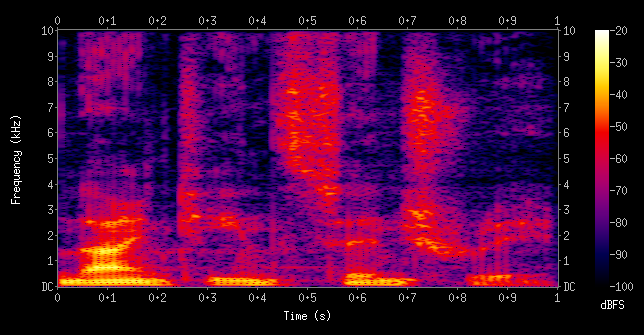
\includegraphics[width=\textwidth]{audio_spectr.png}
    \caption{Аудио спектрограмма спокойного произношения слов
    "nineteenth century"\,(перевод на рус. "девятнадцатый век").}
    \label{fig:audio_spectr}
\end{figure}


\paragraph{Компьютерное зрение}
Другим и крайне важным приложением нейронных сетей является
компьютерное зрение. Две наиболее важные использующиеся технологии это
машинное обучение, а конкретно, глубокое обучение и сверточная
нейронная сеть, которая помогает модели машинного обучения
"вглядываться", разбивая изображения на пиксели и присваивая им метки.
Подобно тому как это делает человек, нейронная сеть сначала различает
четкие края и простые формы, а затем заполняет информацию по мере
выполнения итераций своих прогнозов. Сверточная нейронная сеть
используется для обработки отдельных изображений, в то время как
рекуррентная нейронная сеть аналогичным образом используется в
обработке нескольких кадров связанные друг с другом. На рис.
\ref{fig:comp_vision}
приведен снимок того, как нейронная сеть распознает дорогу.
Последовательно применяя к текущему кадру разные фильтры, она пытается
выделить предмет, разбить его на пиксели и обработать эти данные на
основе пройденного обучения.

\begin{figure}[!htb]
    \centering
    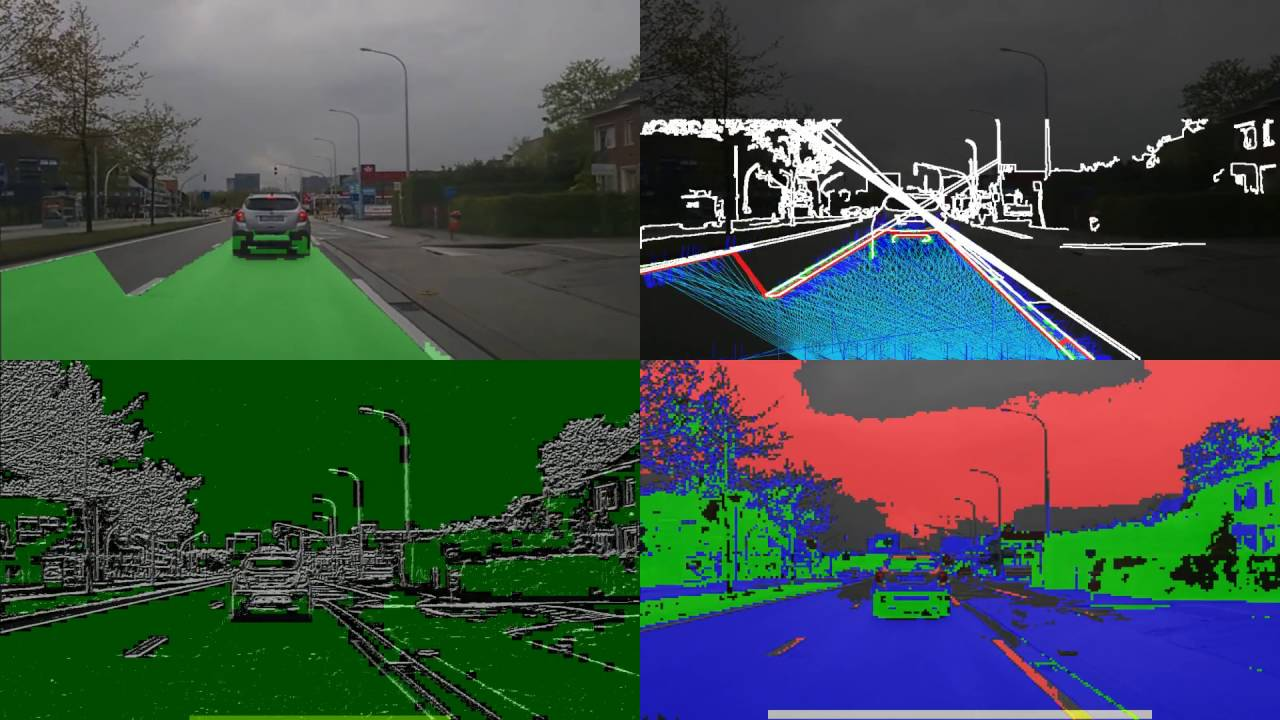
\includegraphics[width=\textwidth]{comp_vision.jpg}
    \caption{Распознавание дороги с помощью компьютерного
    зрения}
    \label{fig:comp_vision}
\end{figure}

\chapter{Самоорганизующиеся карты Кохонена}
\section{Введение} \label{sec:SOM intro}
\textit{Карты самоорганизации} - это особый класс нейронных сетей,
основанный на конкурентном обучении. Нейроны выходного слоя
соревнуются за право активации и в результате каждому входному
сигналу (входному вектору) соответствует лишь один активированный
нейрон (\textit{нейрон-победитель}).

В картах самоорганизации нейроны помещаются в узлах решетки, обычно
одно- или двухмерной. Достаточно редко можно встретить карты более
высоких размерностей. Во время конкурентного процесса нейроны
избирательно настраиваются на различные входные образы или классы
входных образов, организуя тем самым положения нейронов-победителей, а
координаты нейронов решетки являются индикаторами встроенных
статистических признаков, содержащихся в примерах. Т.е. во время
обучения решетка нейронов деформируется в соответствии с изменение
координат нейронов, которые стремятся в точки сгущения признаков и в
идеале каждому признаку соответствует некоторый нейрон в решетке,
который активируется, когда во входном векторе преобладает этот
признак. Отсюда берет свое происхождение и само название
"самоорганизующиеся карты".

Основной целью карт самоорганизации является преобразование
поступающих сигналов, имеющих произвольную размерность, в одно- или
двухмерную дискретную карту (см. рис. \ref{fig:som models}). Помимо
этого, они выполняют
задачу первоначальной разведки данных, выделении признаков, сжатии,
классификации или кластеризации данных перед тем как другие виды
нейронных сетей обученные с учителем на выделенных с помощью
самоорганизующихся карт классов признаков, начнут свою работу.

\section{Структура сети и ее обучение}
В разделе \ref{sec:SOM intro} была введена идея работы
самоорганизующейся карты и теперь можно сделать следующий важный
вывод.
\begin{quote}
    Пространственное положение выходных нейронов в топографический
    карте соответствует конкретной области признаков данных,
    выделенных из входного пространства.
\end{quote}
Откуда следует, что нейроны, работающие с близко расположенными
областями информации, также расположены достаточно близко друг к
другу, таким образом взаимодействуя друг с другом посредством коротких
синаптических связей.

На рис. \ref{fig:som models} показаны две основные модели отображения
признаков, оранжевым цветом выделены нейроны-победители. В
нашей работе будет рассмотрена именно вторая - модель Кохонена,
которая по сравнению с моделью Уилшоу-ван дер Мальсбурга является
более общей в том смысле, что она способна осуществлять сжатие данных
(т.е. уменьшение размерности входного сигнала).

\begin{figure}[!htb]
    \centering
    \subfloat[Модель Уилшоу-ван дер Мальсбурга
    \label{fig:Malsburg Model}]{%
        \resizebox{0.55\paperwidth}{!}{%
        \begin{tikzpicture}
        \draw[fill=white, draw=black, dashed]
        (-3,1) -- (-2,4) -- (2.5, 4) -- (1.5, 1) -- cycle;

        \foreach \u in {0, 1, 2, 3}
        {
            \node[ellipse,
                draw=black,
                fill=gray!20,
                minimum width = 5mm,
                minimum height = 2mm]
            (e12\u) at (-2+1/3+\u*1.15, 3.5) {};

            \node[ellipse,
                draw=black,
                fill=gray!20,
                minimum width = 5mm,
                minimum height = 2mm]
            (e11\u) at (-2+\u*1.15,2.5) {};

            \node[ellipse,
                draw=black,
                fill=gray!20,
                minimum width = 5mm,
                minimum height = 2mm]
            (e10\u) at (-2-1/3+\u*1.15,1.5) {};
        }

        \node[ellipse,
            draw=Orange,
            fill=orange!50,
            minimum width = 5mm,
            minimum height = 2mm]
        (ew) at (-2+1.15,2.5) {};

        \draw[fill=white, draw=black, dashed]
        (-2,-3) -- (0,-1) -- (4,-1) -- (2,-3) -- cycle;

        \foreach \u in {0,1,2,3}
        {
            \node[ellipse,
                draw=black,
                fill=gray!20,
                minimum width = 5mm,
                minimum height = 2mm]
            (e22\u) at (0.06+\u*0.9, -1.5) {};

            \node[ellipse,
                draw=black,
                fill=gray!20,
                minimum width = 5mm,
                minimum height = 2mm]
            (e21\u) at (-0.44+\u*0.9,-2) {};

            \node[ellipse,
                draw=black,
                fill=gray!20,
                minimum width = 5mm,
                minimum height = 2mm]
            (e20\u) at (-0.94+\u*0.9,-2.5) {};
        }

        \node[ellipse,
            draw=Orange,
            fill=orange!50,
            minimum width = 5mm,
            minimum height = 2mm]
        (ea) at (-0.44+1*0.9,-2) {};

        \foreach \u in {0,1,2,3} {
            \foreach \v in {0,1,2}
            {
                \draw[-] (e212) -- (e1\v\u) {};
            }
        }

        \draw[thick, decorate, decoration={calligraphic brace}]
        (-3.2,1) -- (-3.2,4);

        \draw[thick, decorate, decoration={calligraphic brace}]
        (-3.2,-3) -- (-3.2,-1);

        \node[text width = 4cm, align=center] at (-5.3,2.5)
        {Постсинаптические нейроны};

        \node[text width = 4cm, align=center] at (-5.3,-2)
        {Предсинаптические нейроны};

        \node[text width=2.5cm, align=center] at (2.6,0)
        {Пучок связей};
        \end{tikzpicture}
        }
    }
    \hspace{10pt}
    \centering
    \subfloat[Модель Кохонена \label{fig:Kohonen Model}]{%
        \resizebox{0.50\paperwidth}{!}{%
        \begin{tikzpicture}
        \draw[fill=white, draw=black, dashed]
        (-3,1) -- (-2,4) -- (2.5, 4) -- (1.5, 1) -- cycle;

        \foreach \u in {0, 1, 2, 3}
        {
            \node[ellipse,
                draw=black,
                fill=gray!20,
                minimum width = 5mm,
                minimum height = 2mm]
            (e12\u) at (-2+1/3+\u*1.15, 3.5) {};

            \node[ellipse,
                draw=black,
                fill=gray!20,
                minimum width = 5mm,
                minimum height = 2mm]
            (e11\u) at (-2+\u*1.15,2.5) {};

            \node[ellipse,
                draw=black,
                fill=gray!20,
                minimum width = 5mm,
                minimum height = 2mm]
            (e10\u) at (-2-1/3+\u*1.15,1.5) {};
        }

        \node[ellipse,
            draw=Orange,
            fill=orange!50,
            minimum width = 5mm,
            minimum height = 2mm]
        (ew) at (-2+1.15,2.5) {};

        \node[ellipse,
            draw=Green,
            fill=green!50,
            minimum width = 5mm,
            minimum height = 2mm]
        (ea1) at (0.5,-1) {};

            \node[ellipse,
            draw=Green,
            fill=green!50,
            minimum width = 5mm,
            minimum height = 2mm]
        (ea2) at (-1.5,-1) {};

        \foreach \u in {0,1,2,3} {
            \foreach \v in {0,1,2}
            {
                \draw[-] (ea1) -- (e1\v\u) {};
                \draw[-] (ea2) -- (e1\v\u) {};
            }
        }

        \path (ea1) -- (ea2) node [black, font=\large, midway]
        {$\cdots$};

        \draw[thick, decorate, decoration={calligraphic brace}]
        (-3.2,1) -- (-3.2,4);

        \node[text width = 4cm, align=center] at (-5.3,2.5)
        {Постсинаптические нейроны};

        \node[text width = 3cm, align=center] at (-0.4,-1.7)
        {Входной сигнал};

        \node[text width=2.5cm, align=center] at (1.7,0)
        {Пучок связей};
        \end{tikzpicture}
        }
    }
    \caption{Основные модели самоорганизующихся карт}
    \label{fig:som models}
\end{figure}

Алгоритм, ответственный за формирование самоорганизующейся карты,
начинается с инициализации синаптических весов сети. Обычно это
происходит с помощью назначения синаптическим весам малых случайных
значений. При таком формировании карта признаков изначально не имеет
какого-либо порядка признаков. После корректной инициализации сети для
продолжения формирования карты самоорганизации запускаются три
следующих основных процесса.
\begin{enumerate}
    \item \textit{Конкуренция}. Для каждого входного образа нейроны
        сети вычисляют относительные значения дискриминантной функции.
        Эта функция является основной для конкуренции среди нейронов.
    \item \textit{Кооперация}. Победивший нейрон определяет
        пространственное положения топологической окрестности
        нейронов, обеспечивая тем самым базис для кооперации между
        этими нейронами.
    \item \textit{Синаптическая адаптация}. Последний механизм
        позволяет возбужденным нейронам увеличивать собственные
        значения дискриминантных функций по отношению к входным
        образам посредством соответствующих корректировок
        синаптических весов. Корректировки производятся таким образом,
        чтобы отклик нейрона-победителя на последующее применение
        аналогичных примеров усиливался.
\end{enumerate}

\paragraph{Процесс конкуренции}
Пусть $m$ - размерность входного пространства, а входной вектор
выбирается из этого входного пространства случайно и обозначается так:
\begin{equation}
    \bldx =  \left[ x_1, x_2, \dots, x_m \right]^{T}.
\end{equation}
Вектор синаптических весов каждого из нейронов сети имеет ту же
размерность, что и входное пространство. Обозначим синаптический вес
нейрона $j$ следующим образом:
\begin{equation}
    \bldw_j = \left[ w_{j1}, w_{j2}, \dots, w_{jm} \right]^{T},\
    j=\overline{1,l},
\end{equation}
где $l$ - общее количество нейронов сети. Для того, чтобы подобрать
наилучший вектор весов $\bldw_j$, соответствующий входному вектору
$\bldx$, нужно сравнить скалярные произведения $\bldw_j^{T}\bldx$ для
$j=\overline{1,l}$ и выбрать наибольшее значение. При этом
предполагается, что ко всем нейроном применяется некоторое значение
\textit{насыщения}, равное порогу, взятому с противоположным знаком.
Это делается для того, чтобы дополнительно выделить нейрон, который
должен быть активирован и избежать неограниченного наращивания
синаптических весов, которое может привести к неустойчивости системы.
Таким образом, выбирая нейрон с наибольшим скалярным произведением
$\bldw_j^{T}\bldx$, мы в результате определяем местоположение, которое
должно стать центром топологической окрестности возбужденного нейрона.

Применим некоторую хитрость. Максимизация скалярного произведения
$\bldw_j^{T}\bldx$, математически эквивалентна минимизации евклидова
расстояния между векторами $\bldx$ и $\bldw_j$. Тогда если
использовать индекс $i(\bldx)$ для идентификации того нейрона, который
лучше всего соответствует входному сигналу $\bldx$, то эту величину
можно определить с помощью следующего соотношения:
\begin{equation}
    i(\bldx) = \argmin_{1\leqslant j\leqslant l}{\norm{\bldx - \bldw_j}} =
    \sqrt{\sum_{k=1}^{m}{\left|x_k-w_{kj}\right|^{2}}}.
\end{equation}

Конкретный нейрон $i$, удовлетворяющий данному условию, называется
\textit{победившим}.

\paragraph{Процесс кооперации}
Нейрон-победитель находится в центре топологической окрестности
сотрудничающих нейронов, он является возбужденным нейроном, а такие
нейроны всегда стремятся возбудить пространственно близкие к нему
нейроны. Дадим определение топологической окрестности победившего
нейрона $i$, которая плавно уменьшается при удалении от своего центра.
Обозначим символом $h_{j,i}$, топологическую окрестность с центром в
победившем нейроне $i$, состоящую из множества возбуждаемых нейронов,
каждый из которых имеет некоторый индекс $j$. Пусть $d_{j,i}$
расстояние между победившим нейроном $i$ и вторично возбужденным
нейроном $j$, определим значение этого расстояния чуть-чуть позже.
Тогда можно предположить, что топологическая окрестность
$h_{j,i}$ удовлетворяет следующим требованиям.
\begin{itemize}
    \item[$\bigcdot$] Топологическая окрестность $h_{j,i}$ является
        симметричной относительно точки максимума, определяемой при
        $d_{j,i} = 0$ (максимум функции достигается в победившем
        нейроне, т.е. когда $i = j$).
    \item[$\bigcdot$] Амплитуда топологической окрестности $h_{j,i}$
        монотонно уменьшается с увеличением расстояния $d_{j,i}$,
        достигая нуля при $d_{j,i} \to \infty$. Это необходимое
        условие сходимости.
\end{itemize}

Типичным примером такой функции служит функция Гаусса:
\begin{equation} \label{eq:Gauss Func}
    h_{j,i(\bldx)}=\exp{\left(-\frac{d_{j,i(\bldx)}^{2}}{2\sigma^2}\right)}.
\end{equation}

Это выражение является инвариантным к расположению победившего
нейрона (т.е. не зависит от его расположения). Параметр $\sigma$
называется \textit{эффективной шириной} топологической окрестности.
Этот параметр определяет уровень, до которого нейроны из
топологической окрестности победившего участвуют в процессе обучения
(см. рис. \ref{fig:effective width}).
\begin{figure}
    \centering
    \begin{tikzpicture}
        \begin{axis}[
            title={Функция Гаусса, $h(d,\sigma(n))$},
            xlabel={расстояние, $d$},
            ylabel={$h(d,\sigma(n))$},
            grid=major
        ]
            \addplot[
                domain= -30:30,
                very thick,
                smooth,
                Purple
            ]{exp(-(x^2)/(2*2^2))};
            \addlegendentry{$\sigma = 2$};

            \addplot[
                domain= -30:30,
                thick,
                smooth,
                Green,
            ]{exp(-(x^2)/(2*4^2))};
            \addlegendentry{$\sigma = 4$};

            \addplot[
                domain= -30:30,
                thick,
                smooth,
                Red,
            ]{exp(-(x^2)/(2*8^2))};
            \addlegendentry{$\sigma = 8$};

            \addplot[
                domain= -30:30,
                thick,
                smooth,
                Blue
            ]{exp(-(x^2)/(2*10^2))};
            \addlegendentry{$\sigma = 10$};
        \end{axis}
    \end{tikzpicture}
    \caption{Зависимость функции Гаусса от эффективной ширины}
    \label{fig:effective width}
\end{figure}

Для обеспечения кооперации между соседними нейронами необходимо, чтобы
топологическая окрестность $h_{j,i}$ была зависимой от латерального
расстояния между победившим $i$ и возбуждаемым $j$ нейроном в выходном
пространстве. Именно это свойство отражено в выражении \eqref{eq:Gauss Func}.
В случае одномерной решетки расстояние $d_{j,i}$ является целым
числом равным модулю $\left| j-i\right|$. В случае двумерной решетки
это расстояние определяется соотношением
\begin{equation}
    d_{j,i}^{2} = \norm{\bldr_j - \bldr_i}^2,
\end{equation}
где дискретный вектор $\bldr_j$ определяет позицию возбуждаемого
нейрона, а $\bldr_i$ - победившего нейрона. Оба этих измерения
проводятся в дискретном выходном пространстве.

Еще одним уникальным свойством алгоритма обучения самоорганизующейся
карты является то, что размер топологической окрестности со временем
уменьшается. Это требование удовлетворяется за счет постепенного
уменьшения ширины $\sigma$. Например, можно уменьшать ее
экспоненциально в зависимости от дискретного времени $n$ (см. рис.
\ref{fig:effective width 2}):
\begin{equation}
    \sigma(n) = \sigma_0\exp{\left( - \frac{n}{\tau_1}\right)},\, n
    \in \NN,
\end{equation}
где $\sigma_0$ - начальное значение величины $\sigma$; $\tau_1$ -
некоторая константа.

\begin{figure}
    \centering
    \begin{tikzpicture}
        \begin{axis}[
            title={Эффективная ширина, $\sigma(n)$},
            xlabel={шаг, $n$},
            ylabel={$\sigma(n)$},
            grid=major,
            % xmin=0,ymin=0,
            % xmax=4000,ymax=12,
            % xtick=500,ytick=2
        ]
            \addplot[
                domain=0:4000,
                ultra thick,
                Purple,
                samples=200,
            ]{10*exp(-((x)/(1000/log10(10)))};

        \end{axis}
    \end{tikzpicture}
    \caption{Пример изменения функции эффективной ширины с течением
    времени}
    \label{fig:effective width 2}
\end{figure}

По окончании этапа обучения функция $h_{j,i}$ должна охватывать только
ближайших соседей. Исходя из этого мы получаем следующую форму функции
топологической окрестности:
\begin{equation}
    h_{j,i(\bldx)}(n) = \exp\left( -\frac{d_{j,i}^{2}}{2\sigma^2(n)} \right),\ n \in \NN.
\end{equation}
Таким образом, при увеличении количества итераций $n$ ширина
$\sigma(n)$ экспоненциально убывает, а вместе с ней соответственно
сжимается и топологическая окрестность см. рис. \ref{fig:h educ}.

\begin{figure}[!htb]
    \centering
    \subfloat[До обучения \label{fig:educ before}]{%
            \begin{tikzpicture}
                \begin{axis}[
                    domain=-10:9,
                    mesh,
                    % colormap/PuBu,
                    grid=major,
                ]
                    \addplot3[surf]{exp(-(x^2+y^2)/30)};
                \end{axis}
        \end{tikzpicture}
    }
    \subfloat[После обучения\label{fig:educ after}]{%
            \begin{tikzpicture}
                \begin{axis}[
                    grid=major,
                ]
                    \addplot3[surf]{exp(-(x^2+y^2)/2)};
                \end{axis}
        \end{tikzpicture}
    }
    \caption{Изменение топологической окрестности нейрона до и после
    обучения сети}
    \label{fig:h educ}
\end{figure}

\paragraph{Процесс адаптации}
Процесс синаптической адаптации включает в себя изменение
синаптических весов сети. Для того, чтобы сеть могла
самоорганизоваться, вектор синаптических весов $\bldw_j$ нейрона j
должен изменяться в соответствии с входным вектором $\bldx$.
Заметим, что изменения в связях происходит только в одном направлении,
что в конечном счете приводит все веса к точке насыщения. Для того,
чтобы обойти эту проблему введем функцию забывания $g(y_i)\bldw_j$.
Единственным требование, налагаемым на эту функцию станет равенство
\begin{equation} \label{eq:gy}
    g(y_i) = 0,\ \text{при}\ y_i = 0.
\end{equation}

Имея такую функцию, изменение вектора весов нейрона $j$ в решетке
можно выразить следующим образом:
\begin{equation} \label{eq:delta w 1}
    \Delta\bldw_j = \eta y_i\bldx - g(y_i)\bldw_j,
\end{equation}
где, $\eta$ - параметр скорости обучения алгоритма. Для удовлетворения
условия \eqref{eq:gy} выберем следующую линейную функцию $g(y_i)$:
\begin{equation}
    g(y_i) = \eta y_i.
\end{equation}

Теперь для упрощения выражения \eqref{eq:delta w 1} примем $y_j =
h_{j,i(\bldx)}$ и получим формулу изменения матрицы весов:
\begin{gather}
    \Delta\bldw_j = \eta h_{j,i(\bldx)}\cdot(\bldx - \bldw_j);\\
    \bldw_j(n+1) = \bldw_j(n) +
    \eta(n)h_{j,i(\bldx)}(n)(\bldx-\bldw_j(n)).
\end{gather}

Это выражение применяется ко всем нейронам решетки, которые лежат в
топологической окрестности победившего нейрона $i$.


\vspace{5mm}
Таким образом, представленный алгоритм ведет к топологическому
упорядочиванию пространства признаков во входном пространстве.

\chapter{Реализация}
Перейдем к реализации самоорганизующейся карты Кохонена. Для начала
реализуем структуру, которая будет представлять вычислительный нейрон.
Как обсуждалось ранее в разделе \nameref{sec:neuron models} общем
случае вычислительный нейрон описывается набором синаптических связей,
сумматором и функцией активации. Но поскольку нам нужно описать нейрон
в модели самоорганизующейся карты, то для описания нейрона потребуется
только синаптические связи и его координаты на \textit{карте свойств}
(выходной слой). Кроме того дальше нам необходимо вычислять расстояние
между нейронами в том пространстве, где они находятся, конкретно, в
этом пространстве будет определена евклидова норма, порождающая в нем
евклидову метрику. Кроме того нет смысла усложнять описание этой
структуры приватными полями и структурами, поэтому достаточно будет
реализовать именно \verb|struct neuron|. Итак необходимый нам
вычислительный нейрон может быть представлен структурой описанной в
листинге \ref{code:neuron}.

\begin{listing}[!ht]
    \inputminted{cpp}{code/struct_neuron.hpp}
    \caption{Реализация вычислительного нейрона карты}
    \label{code:neuron}
\end{listing}

Дальше нам понадобиться определять равные между собой нейроны и
определять меньший из них, поэтому так же реализуем нужные бинарные
операции сравнения см. листинг \ref{code:comp_neuron}.

\begin{listing}[!ht]
    \inputminted{cpp}{code/comp_neuron.hpp}
    \caption{Бинарные операций сравнения \textbf{struct neuron} }
    \label{code:comp_neuron}
\end{listing}

Начнем реализовывать структуру для описания самой карты. Поскольку
к каждому типу нейронной сети необходим индивидуальный подход нет
смысла создавать лишние абстракции и использовать ненужные здесь
механизмы наследования. Давайте начнем реализовать наш
\verb|class sokm| см. листинг \ref{code:base_sokm}.

\begin{listing}
    \inputminted{cpp}{code/base_sokm.hpp}
    \caption{Код части реализации \textbf{class sokm} }
    \label{code:base_sokm}
\end{listing}

Обновление введенных констант будет происходить с помощью функций
представленные в листинге \ref{code:constants_update}.

\begin{listing}
    \inputminted{cpp}{code/utils.hpp}
    \caption{Код реализующий обновление констант}
    \label{code:constants_update}
\end{listing}

Мы обсудили, что процесс обучения нейронной сети сводится к основным
модулям процессу адаптации, процессу кооперации и процессу адаптации
каждый из них может быть реализован по отдельности как показано в
листинге \ref{code:train_less}.

\begin{listing}
    \inputminted{cpp}{code/train_less.hpp}
    \caption{Раздельная реализации основных этапов обучения сети}
    \label{code:train_less}
\end{listing}

Однако в целях улучшения производительности кода мы поместим
реализации процессов кооперации и адаптации в одну функцию
\verb|train()|, показанную в листинге \ref{code:train}. Она же и станет
основной функцией обучения нашей самоорганизующейся карты.

\begin{listing}
    \inputminted{cpp}{code/train.hpp}
    \caption{Реализации функции \textbf{train()}}
    \label{code:train}
\end{listing}

Для вычисления топологической окрестности нейрона использовалась
функция \verb|hji()|, а для вычисления квадрата евклидова расстояния
между вектор входного сигнала и вектором весом использовалась функция
\verb|sq_euclidean_distance()|. Обе эти функции представлены в листинге
\ref{code:hji}.

\begin{listing}
    \inputminted{cpp}{code/train.hpp}
    \caption{Реализации функций \textbf{hji()} и \textbf{sq\_euclidean\_distance()}}
    \label{code:hji}
\end{listing}

Реализации чтения данных для обучения и места входа программы (\verb|main()|)
представлены в листингах \ref{code:full_sokm}
и \ref{code:full_main} в разделе \nameref{sec:appendix}.

\chapter{Заключение}


\chapter{Приложение} \label{sec:appendix}

\begin{listing}
    \inputminted{cpp}{code/utils.hpp}
    \caption{Полный код реализации вспомогательных пространств имен}
    \label{code:full_utils}
\end{listing}

\begin{listing}
    \inputminted{cpp}{code/sokm.hpp}
    \caption{Полный код реализации \textbf{struct neuron} и \textbf{class sokm}}
    \label{code:full_sokm}
\end{listing}

\begin{listing}
    \inputminted{cpp}{code/main.cpp}
    \caption{Полный код основной вызывающей функции \textbf{main()}}
    \label{code:full_main}
\end{listing}

\end{document}
